\chapter{Estado del arte}\label{sec:Estado_arte}
\section{Robótica, drones}
Un dron se puede definir como una \textit{aeronave} pilotada de forma remota. El uso de los drones se ha ido instaurando poco a poco en la sociedad; actualmente con sus nuevas mejoras y reducido coste, estos han pasado de una situación en la que era más “amateur” a una función más profesional. En los últimos años han estado cada vez más presentes ya que ofrecen una gran herramienta de trabajo para diferentes sectores tanto comerciales como de seguridad. 

\subsection{Evolución histórica}
La palabra inglesa \textit{drone} (dron en español) tiene varios significados, aunque en su origen \textit{drone} se refiere a los zánganos de las colmenas y al zumbido que emiten. El ruido que se escucha en tierra cuando vuelan a cierta altura estos vehículos recordaba a estos zánganos y de ahí que se quedaran con este nombre. Su evolución proviene sobretodo en el ámbito militar dónde tenían funciones de reconocimiento y permitían tener ventaja en la batalla.\newline 

El inicio de los primeros vehículos no tripulados se remonta a la Primera Guerra Mundial . Estos primeros modelos fueron lanzados por catapulta o volados usando radio control. En enero de 1918, el ejército de los Estados Unidos comenzó la producción de torpedos aéreos teleridigidos de forma remota; desarrollando lo que podemos considerar el primer dron de la historia, el Kettering Bug (figura \ref{fig:Kettering Bug}). El Kettering Bug fue volado con éxito en algunas pruebas; sin embargo aunque la guerra terminó antes de que pudiera desarrollarse más, marcó el inicio de la revolución de los drones . \newline 

\begin{figure}[H]
	\center
	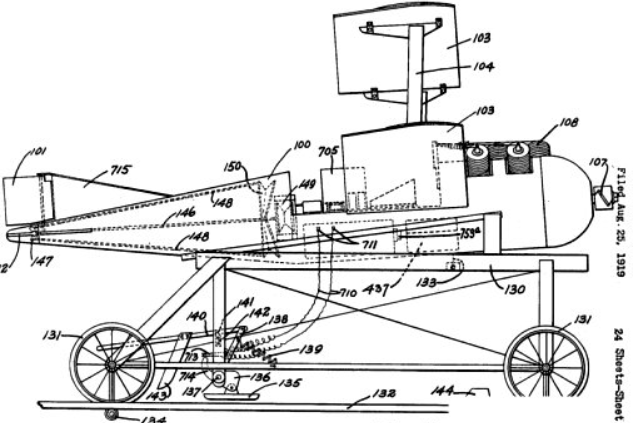
\includegraphics[scale=0.5]{imagenes/EstadodelArte/ketbug.png}
	\caption{Patente del Kettering Bug}
	\label{fig:Kettering Bug}
\end{figure}
 
Los drones que conocemos hoy en día eran llamados \textit{UAV} (Vehículos aéreos no tripulados). Los UAV con fines de reconocimiento se desplegaron por primera vez a gran escala en la Guerra de Vietnam. En esta época también comenzaron a usarse en una variedad de nuevos roles, como actuar de señuelos en combate, lanzar misiles contra objetivos fijos y lanzar folletos para operaciones psicológicas. 

Después de la Guerra de Vietnam, otros países fuera de Gran Bretaña y Estados Unidos comenzaron a explorar la tecnología de los \textit{UAV}. Los nuevos modelos se volvieron más sofisticados, con una resistencia mejorada y la capacidad de mantener una mayor altura. En los últimos años, se han desarrollado modelos que utilizan tecnología como la energía solar para abordar el problema de alimentar vuelos más largos. \newline

Los drones ahora tienen muchas funciones, que van desde monitorear el cambio climático hasta llevar a cabo operaciones de búsqueda después de desastres naturales, fotografía, filmación y entrega de bienes. Pero su uso más conocido y controvertido es el uso militar para reconocimiento, vigilancia y ataques dirigidos. Desde los atentados terroristas del 11 de septiembre, Estados Unidos aumentó significativamente el uso de drones, aplicándose posteriormente a un nivel global para la seguridad. Se utilizan principalmente para la vigilancia en áreas y terrenos donde las tropas no pueden ir con seguridad; aunque, tristemente también tienen un gran potencial ofensivo. \newline \cite{HistDrones} \cite{HistDrones2}


\subsection{Tipos}

Los drones están en su punto más alto y cada vez son más las empresas que definen sus productos como \textit{drones} , por lo que existe un gran abanico de posibilidades en cuanto a su clasificación. \cite{TipoDron} Sin embargo la más extendida son \textbf{según su uso} y \textbf{según el tipo de ala.} \newline

Según su uso: 

\begin{itemize}
	\item \textbf{Uso Militar.} Se usan con fines de reconocimiento, como ofensiva e incluso reabastecimiento de provisiones. En este campo se pueden incluir los usados por la policía.
	\item \textbf{Uso Comercial.} Se encuentran desde los usados como diversión hasta los usados para publicidad,etc.
\end{itemize}

Según el tipo de ala:

\begin{itemize}
	\item \textbf{Drones de ala fija \ref{fig:Alafija}.} Estos drones proporcionan una gran autonomía durante el vuelo ya que son muy aerodinámico; sin embargo necesitan mucho espacio para aterrizar y un sistema de lanzado para despegar, lo que los hace muy engorrosos. Se utilizan sobre todo para hacer mapas y labores de riego
\begin{figure}[H]
	\center
	\includegraphics[scale=0.125]{imagenes/EstadodelArte/Alafija.png}
	\caption{Ala fija}
	\label{fig:Alafija}
\end{figure}
 
	\item \textbf{Drones de ala rotatoria\ref{fig:Alarotatoria}.} Son los más extendidos en el ámbito comercial. A diferencia con los de ala fija estos pueden permanecer suspendidos en el aire gracias al sistema de hélices que llevan; no obstante tienen mucha menos autonomía que los de ala fija haciéndolos útiles solo para vuelos cortos. Cómo se pueden mantener estables gracias a sus giroscopios y estabilizadores son ideales para sacar fotos y hacer vídeos.
\begin{figure}[H]
	\center
	\includegraphics[scale=0.1]{imagenes/EstadodelArte/Alarotatoria.png}
	\caption{Ala rotatoria}
	\label{fig:Alarotatoria}
\end{figure}
 
\end{itemize}

Dentro de cada tipo, cada dron cuenta con un receptor radio determinado. A la hora de elegir el dron para nuestro proyecto será importante mirar las especificaciones del receptor radio que posee, ya que las comunicaciones entre el dron y la emisora (En este caso la FPGA) puede funcionar con distintos protocolos de comunicaciones. 

\subsection{Protocolos de comunicaciones de un dron}\label{sec:comdron}

En el ámbito de los drones, las más importantes son PWM, PPM y PCM.

\subsubsection{Modulación por ancho de pulsos (PWM)}

La modulación por ancho de pulsos o PWM es un método que permite generar una señal analógica desde un sistema digital.  Una señal de PWM es periódica y tiene dos elementos principales: un ciclo de trabajo y una frecuencia. \newline El ciclo de trabajo describe la cantidad de tiempo que la señal está en estado alto, como un porcentaje con respecto a la cantidad de tiempo que está en estado bajo. La frecuencia determina cómo de rápido la señal completa un ciclo, y por lo tanto que tan rápido cambia entre los estados alto y bajo.  Este ciclo de trabajo será modificado para transmitir una información o controlar la energía de la señal enviada, mientras que la frecuencia debe ser siempre la misma para poder medir el tiempo que la señal está en alto. 

\begin{figure}[H]
	\center
	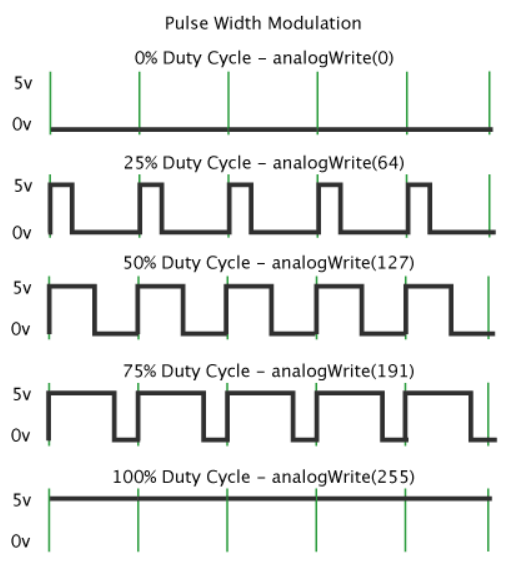
\includegraphics[scale=0.7]{imagenes/EstadodelArte/pwm.png}
	\caption{Modulación PWM}
	\label{fig:PWM}
\end{figure}

Esta modulación se utiliza mucho en la industria(ya que es la más común y generalmente la más barata.), y es con la que se controlan la mayoría de los servos en la robótica. 
Cada canal tiene su propio cable único, por lo que si tiene un receptor de 8 canales necesitará conectar 8 cables para leer las entradas en su controlador de vuelo.

\subsubsection{Modulación de posicion de puntos (PPM)}
En la Modulación por Posición de Pulso o PPM la amplitud y el ancho son fijos, pero la posición del pulso es variable. Es un tipo de modulación en la cual una palabra de M bits se codifica para la transmisión de un pulso que se encuentra en las N posiciones posibles,  donde N corresponde al tipo de modulación PPM (N-PPM).
\begin{equation} 
N=2^M 
\end{equation} 
La ventaja de PPM es que solo se necesita un cable de señal para varios canales (típicamente 8 canales como máximo), en lugar de varios cables individuales. Por lo tanto, solo debe conectar el cable de tierra, alimentación y señal.

\begin{figure}[H]
	\center
	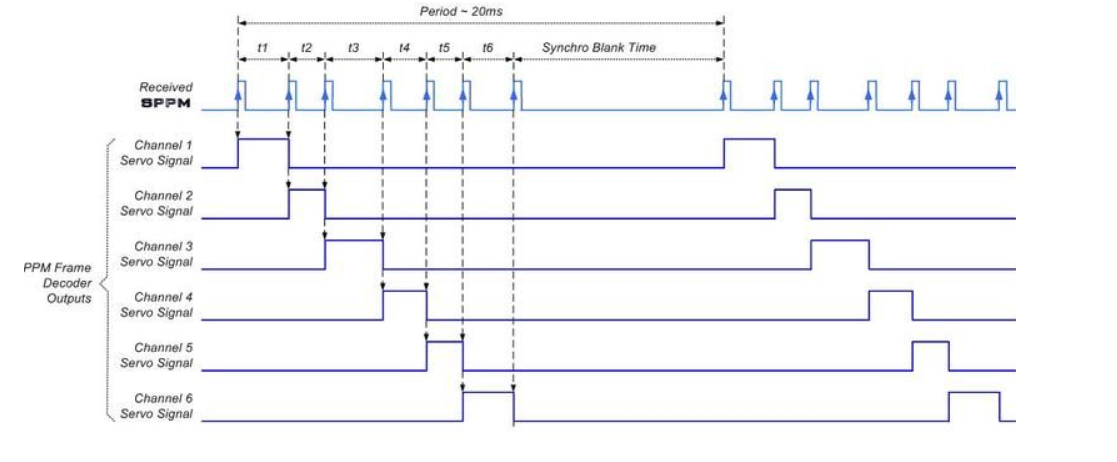
\includegraphics[scale=0.5]{imagenes/EstadodelArte/ppm.png}
	\caption{Modulación PPM}
	\label{fig:PWM}
\end{figure}

\subsubsection{Modulación de código de pulso (PCM)}

La modulación de código de pulso o PCM, es un tipo de modulación similar a PPM; sin embargo, la señal modulada en PCM es una señal digital (usando unos y ceros) mientras que la señal PPM es analógica. La modulación PCM tiene un gran potencial de detección de errores e incluso de corrección, es más confiable y menos susceptible a las interferencias; no obstante, requiere varias conversiones adicionales para su funcionamiento lo que se traduce en equipos muy costosos.


\section{Bioseñales y el EMG}

Entendemos por bioseñal \cite{nait2009advanced} cualquier señal de los seres vivos que se puede medir así como monitorear. Normalmente el término bioseñal se usa para refirse a señales bioeléctricas variantes en el tiempo; pero puede usarse también para señales no eléctricas, como por ejemplo la termografía o la respiración.\newline

Estas bioseñales eléctricas generalmente se caracterizan por un cambio de corriente eléctrica; producido por la diferencia de potencial eléctrico a través de un tejido, órgano o sistema. Entre las más conocidas tenemos: 

\subsubsection{Electrocardiograma}

Un \textit{electrocardiograma} \cite{subramanian2017ecg} (ECG) es el registro de la actividad eléctrica del corazón durante un período de tiempo, utilizado por los médicos para predecir y tratar diversas enfermedades cardiovasculares. Se capta a través de unos electrodos en la piel que detectan la despolarización y repolarización del corazón durante cada latido cardíaco, lo que proporciona una visión de la actividad muscular del corazón. \newline

Un trazado de ECG típico es un ciclo de tres entidades:

\begin{itemize}
	\item \textbf{La onda P}, que representa la despolarización de las aurículas.
	\item \textbf{El complejo QRS}, que representa la despolarización de los ventrículos .
 	\item \textbf{La onda T}, que representa la repolarización de los ventrículos.
\end{itemize}

\begin{figure}[H]
	\center
	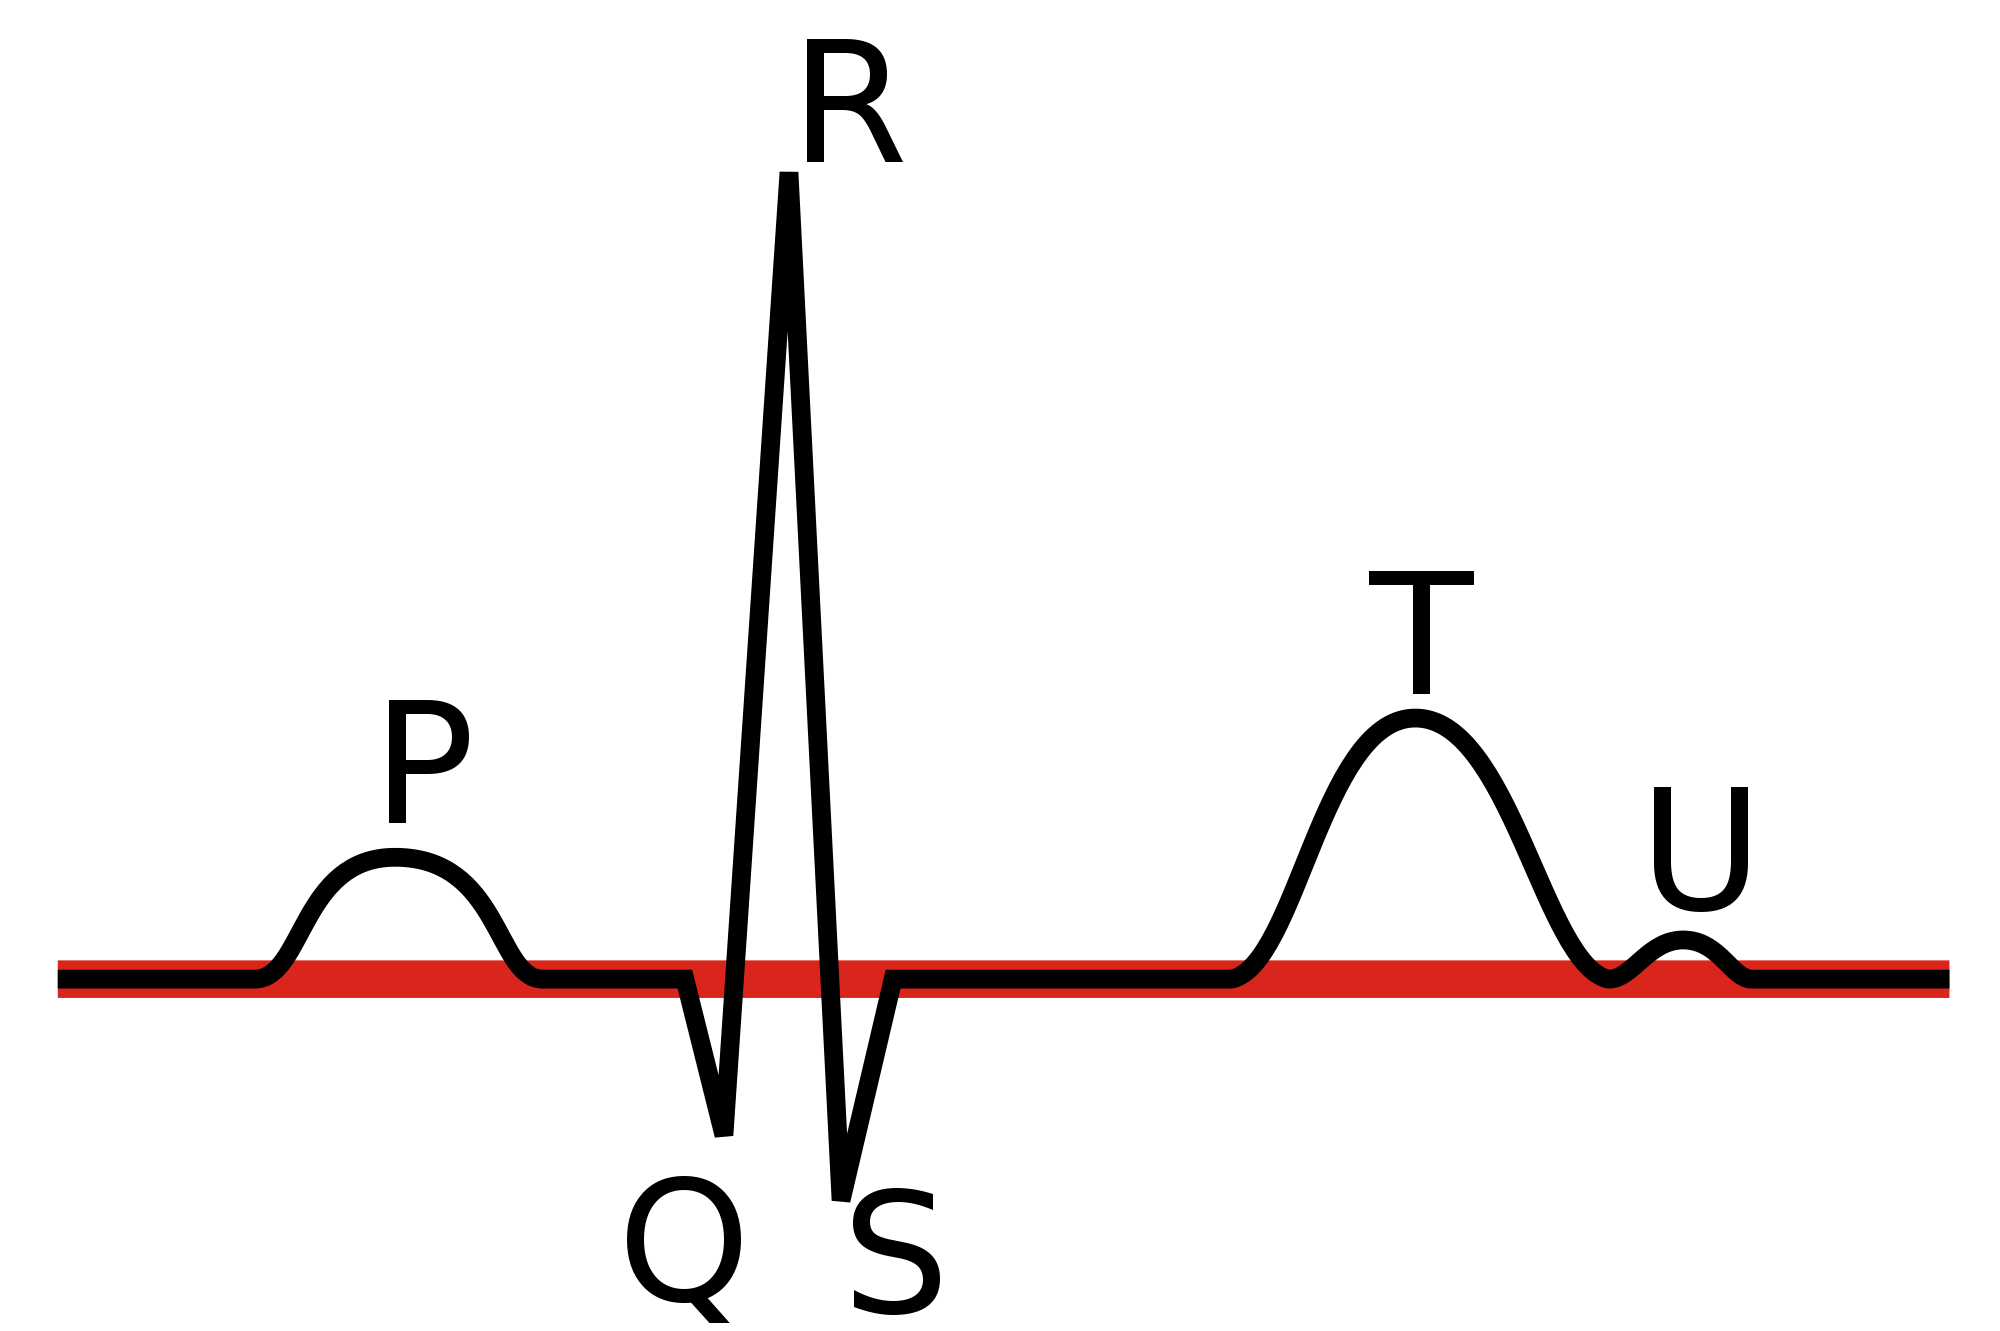
\includegraphics[scale=0.1]{imagenes/EstadodelArte/ECG.png}
	\caption{ECG de un corazón en ritmo sinusal normal}
	\label{fig:ECG}
\end{figure}
 

\subsubsection{Electroencefalografía}

La \textit{electroencefalografía} (EEG) mide la actividad eléctrica del cerebro, registrada a partir de electrodos colocados en el cuero cabelludo. Cuando se analizan estas señales, se utilizan como una herramienta de diagnóstico para detectar patologías asociadas con un comportamiento eléctrico extraño.  Se usa con mayor frecuencia para diagnosticar la epilepsia , lo que causa anormalidades ev en las lecturas del EEG. También se usa para diagnosticar trastornos del sueño , profundidad de la anestesia , coma , encefalopatías y muerte cerebral.

\begin{figure}[H]
	\center
	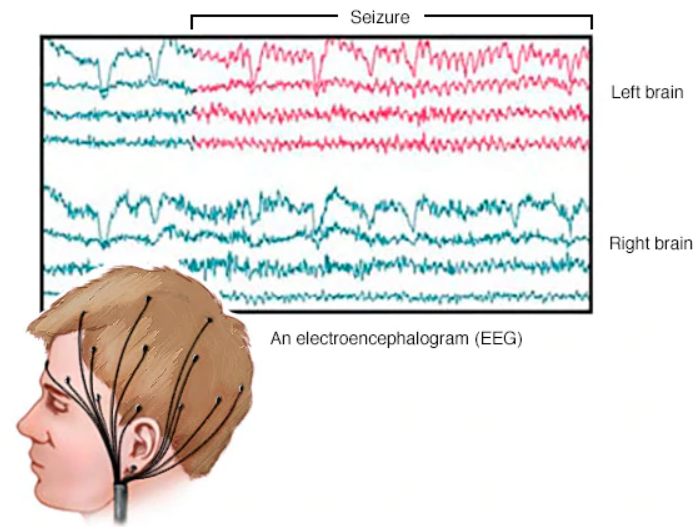
\includegraphics[scale=0.7]{imagenes/EstadodelArte/EEG.png}
	\caption{EEG y colocación de los electrodos}
	\label{fig:EEG}
\end{figure}
 

\subsubsection{Electromiograma}

La \textit{electromiografía} ( EMG ) es una técnica de medicina electrodiagnóstica para evaluar y registrar la actividad eléctrica producida por los músculos esqueléticos . Cada vez que se ejecutan los músculos del cuerpo para una determinada actividad, el cerebro envía señales de excitación a través del \textit{sistema nervioso central}. Los músculos están inervados en grupos llamados \textit{unidades motoras}, que son el punto de unión donde se encuentran la neurona motora y las fibras musculares.  Cuando la \textit{unidades motora} se activa, produce un potencial de acción y el sistema nervioso central se activa continuamente durante el tiempo que se requiera que el músculo genere fuerza. Este \textit{potencial de acción de la unidad motora} es la señal EMG que vemos resultante.

Para obtener el EMG se utiliza un electromiógrafo, el cuál detecta el potencial eléctrico generado por las células musculares cuando estas células se activan eléctrica o neurológicamente. En el ámbito médico por lo tanto el EMG se utiliza como herramienta de diagnóstico para enfermedades neuromusculares, pero sus usos se han ampliado actualmente a la rehabilitación de pacientes en forma de prótesis robótica. \newline

Y es que en nuestros días un mecanismo róbótico con varios grados de libertad puede imitar perfectamente el movimiento de una extremidad humana. 

\begin{figure}[H]
	\center
	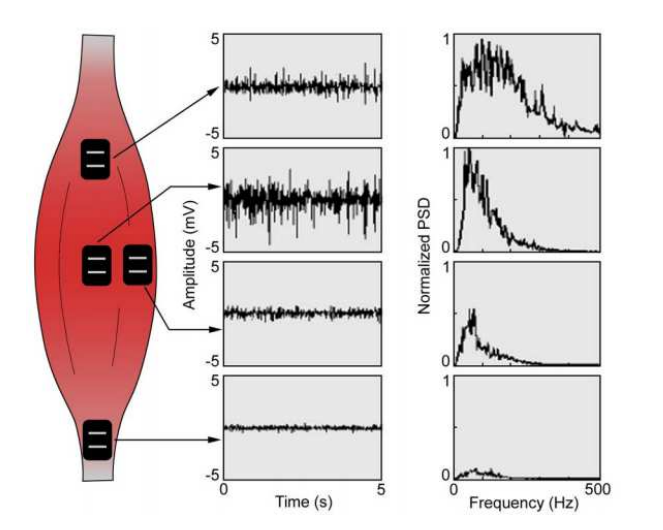
\includegraphics[scale=0.7]{imagenes/EstadodelArte/EMG.png}
	\caption{EMG y colocación de los electrodos}
	\label{fig:EMG}
\end{figure}

Se propone usar la bioseñal EMG en este proyecto debido a la facilidad para discriminar movimientos, que será lo que permita controlar el dron y definir su comportamiento. Sin embargo, antes de poder usar la señal EMG hay que tener varios factores en cuenta, que va desde su captación hasta las posibles interferencias que pueden acusar a este tipo de señal. \ref{sec:Ruido}

\subsection{Tipo de señal y ruido}\label{sec:Ruido}

Antes de pasar a la fase de adquisición de la señal, es importante familiarizarse con los distintos factores que afectan a las propiedades cualitativas de la señal.\newline

Una señal de EMG tiene las siguientes características:
\begin{itemize}
	\item La amplitud de la señal EMG se encuentra entre 1-10 mV, lo que la convierte en una señal considerablemente débil. 
	\item La señal se encuentra en el rango de frecuencia de 0-500 Hz y la más dominante es entre 50-150 Hz.
	\item La señal EMG está muy influenciada por el \textit{ruido:}\newline
	\begin{itemize}
		\item El ruido ambiental puede ser causado por fuentes de radiación electromagnética, por ejemplo, dispositivos de transmisión de radio, luces fluorescentes y la interferencia de la línea de alimentación de los cables eléctricos. Estas interferencias son casi imposibles de evitar por medios externos. Este ruido particular 			existe en el rango de frecuencia de 50-60 Hz. \newline
		\item El ruido también se puede generar a partir de artefactos de movimiento. Las dos fuentes principales de este ruido son la inestabilidad de la interfaz de la capa del electrodo y el movimiento del cable del electrodo y se encuentra principalmente en el rango de 0-20 Hz. Se puede eliminar mediante un conjunto 					adecuado de equipos y circuitos de EMG. La máxima fidelidad de la señal está determinada por la relación señal / ruido EMG adquirida. \newline
	\end{itemize}
\end{itemize}

El kit biosignalplux nos va a permitir adquirir las señales EMG y poder ver la interacción eléctrica en tiempo real. Este kit será el que utilicemos para obtener las señales EMG y procesarlas posteriormente.




